\begin{flushright} {\tiny {\color{gray} \tt pair\_raviart\_thomas.tex}} \end{flushright}
%~~~~~~~~~~~~~~~~~~~~~~~~~~~~~~~~~~~~~~~~~~~~~~~~~~~~~~~~~~~~~~~~~~~~~~~~~~~~~~~~~~~~~~~~~~~~~~~~~~
 
In \textcite{hald03} (2003) we find: 
\begin{displayquote}
{\color{darkgray}
$P_1^\perp \times P_0$ symbol denotes an element with 
normal velocity nodes in the middle of each edge of the
triangulation [...]. This element, also called low order Raviart–Thomas element 
(Raviart and Thomas, 1977), is based on flux conservation on elements edges and 
the resulting scheme is very close to a finite volume scheme.
}
\end{displayquote}

It is mentioned in \textcite{john16}, appendix B.3, example B.45: 
\begin{displayquote}
{\color{darkgray}
the normal component of v 
on each face is a constant. The normal component of functions from RT0 is
continuous across faces of the mesh cells.
}
\end{displayquote}


In \textcite{chen93a} (1993) we read:
\begin{displayquote}
{\color{darkgray}
Arnold and Brezzi [2] showed, for
example, that the Raviart-Thomas mixed method of lowest order is
equivalent to the usual $P_1$-nonconforming method modified by augmenting
the classical $P_1$-nonconforming space with $P_3$-bubbles and then proved that
the equivalence is useful not only for implementing the mixed method but
also for deriving error estimates.
}
\end{displayquote}


There is an entry on Wikipedia\footnote{\url{
https://en.wikipedia.org/wiki/Raviart-Thomas_basis_functions
}} but it is short and not so useful, except for
\begin{displayquote}
{\color{darkgray}
In applied mathematics, Raviart–Thomas basis functions are vector basis functions used 
in finite element and boundary element methods. They are regularly used as basis 
functions when working in electromagnetics. 
}
\end{displayquote}

There is also a useful entry on Stackexchange\footnote{\url{
https://scicomp.stackexchange.com/questions/20245/raviart-thomas-elements-on-reference-square}}:
\begin{displayquote}
{\color{darkgray}
There are quadrilateral Raviart-Thomas elements. 
In two dimensions, the polynomial space for $RT_k$ is given by 
$P_{k+1,k} \times P_{k,k+1}$, where
\[
P_{k,l}=\left\{ \sum_{i=0}^{k} \sum_{j=0}^{l} a_{ij} x^i y^j: a_{ij}\in \R  \right\}
\]

A typical polynomial for $k=0$ would thus be 
\[
\left(
\begin{array}{c}
a_1+b_1 x \\
a_2+b_2 y
\end{array}
\right)
\]
and for $k=1$:
\[
\left(
\begin{array}{c}
a_1+b_1 x +c_1x^2 +d_1 y + e_1 xy  + f_2 x^2 y\\
a_2+b_2 y +c_2y^2 +d_2 x + e_2 xy  + f_2 x y^2
\end{array}
\right)
\]
Hence, $dim(RT_1)=12$, and in general, $dim(RT_k)=2(k+1)(k+2)$. 
This means you need two additional degrees of freedom, which should be located on the 
interior of the element. (In general, for $RT_k$ you take $k+1$ normal derivatives on each facet, 
and the remaining degrees of freedom from the interior.)

For Raviart-Thomas elements, you usually take moments rather than 
point evaluations, i.e., the remaining conditions come from the conditions 
\[
\int_{-1}^{+1} \int_{-1}^{+1} \phi_i(x,y)q_j(x,y)dx dy = \delta_{ij}
\]
where the ${q_j}$ are a basis of $P_{k-1,k}\times P_{k,k-1}$ (e.g. $1,x,y$ for $k=1$).
To make it easier to get a full nodal basis, the facet degrees of freedom are 
usually not taken as point evaluation, but also as moment conditions: 
\[
\int_{e_m} \phi_i(s)^T \nu_{e_m} q_{m,j}(s) ds
\]
where $e_m$ is one of the four edges, $\nu_{e_m}$ is the corresponding outer normal, 
and for each $m$, the $q_{m,j}$ form a basis of $P_k(e_m)$ (e.g. {1,x} or {1,y}
for $k=1$ depending on the edge orientation).
Together, these degrees of freedom are unisolvent (i.e., the corresponding system 
of basis functions is always invertible).
}
\end{displayquote}




- Raviart Thomas 0 RT0 \cite{rath77} ? mentioned/defined/drawn in 4.2.2 of 
Kanschat book. Also exist for quads see 4.2.37

-Check \textcite{brfo}



This element is implemented in deal.ii and we 
read\footnote{\url{https://www.dealii.org/current/doxygen/deal.II/classFE__RaviartThomas.html}}:
\begin{displayquote}
{\color{darkgray}
The Raviart-Thomas space is designed to solve problems in which the solution only 
lives in the space $H^{div}=\{ {\bm u} \in L_2 :div({\bm u}) \in L_2\}$, 
rather than in the more commonly used space $H^1=\{ {\bm u} \in L_2 : \nabla {\bm u} \in L_2 \}$. 
In other words, the solution must be a vector field whose divergence is square integrable, 
but for which the gradient may not be square integrable. The typical application for this space 
(and these elements) is to the mixed formulation of the Laplace equation and related situations, 
see for example step-20. The defining characteristic of functions in  $H^{div}$ is that they are 
in general discontinuous - but that if you draw a line in 2d (or a surface in 3d), 
then the normal component of the vector field must be continuous across the line (or surface) 
even though the tangential component may not be. As a consequence, the Raviart-Thomas element 
is constructed in such a way that (i) it is vector-valued, (ii) the shape functions are 
discontinuous, but (iii) the normal component of the vector field represented by each shape 
function is continuous across the faces of cells.

Other properties of the Raviart-Thomas element are that 
(i) it is not a primitive element ; 
(ii) the shape functions are defined so that certain integrals over the faces are 
either zero or one, rather than the common case of certain point values being 
either zero or one. 

We follow the commonly used - though confusing - definition of the ``degree'' of RT elements. 
Specifically, the ``degree'' of the element denotes the polynomial degree of the 
largest complete polynomial subspace contained in the finite element space, 
even if the space may contain shape functions of higher polynomial degree. 
The lowest order element is consequently FE\_RaviartThomas(0), i.e., 
the Raviart-Thomas element ``of degree zero'', even though the functions of this space 
are in general polynomials of degree one in each variable. This choice of ``degree'' 
implies that the approximation order of the function itself is degree+1, as with usual polynomial spaces. 
}
\end{displayquote}

On the defelement site\footnote{\url{https://defelement.com/elements/raviart-thomas.html}} we find 
that it is defined on triangles, tetrahedra, quadilaterals and hexahedra.
with the number of dofs defined as follows:
\begin{itemize}
\item triangle: $k(k+2)$
\item tetrahedron: $k(k+1)(k+3)/2$
\item quadrilateral: $2k(k+1)$
\item hexahedron: $3k^2(k+1)$
\end{itemize}



\noindent
\underline{\bf Degree 1 Raviart–Thomas on a triangle - Lagrange variant}

\begin{center}
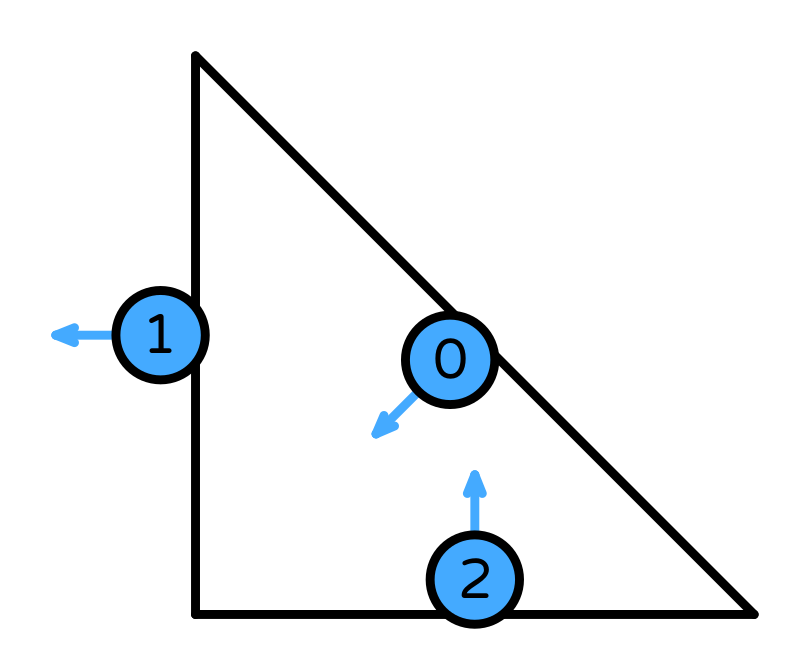
\includegraphics[width=3cm]{images/pair_raviart-thomas/element-Raviart-Thomas-variant-equispaced-triangle-1-dofs-large}\\
{\captionfont Taken from \url{https://defelement.com/}}
\end{center}

${\cal V}$ is a finite dimensional polynomial space on of dimension $n$ and is spanned by 
\[
\left( \begin{array}{c}1 \\ 0  \end{array} \right),
\left( \begin{array}{c}0 \\ 1  \end{array} \right),
\left( \begin{array}{c}x \\ y  \end{array} \right)
\]
Functionals and basis functions:

\begin{center}
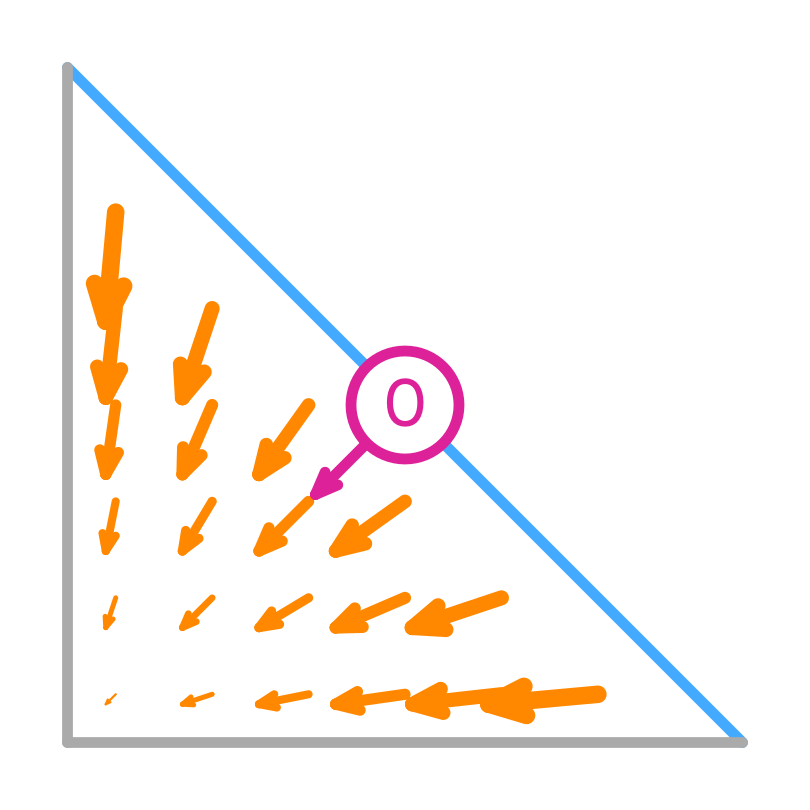
\includegraphics[width=3cm]{images/pair_raviart-thomas/element-Raviart-Thomas-variant-equispaced-triangle-1-0-large}
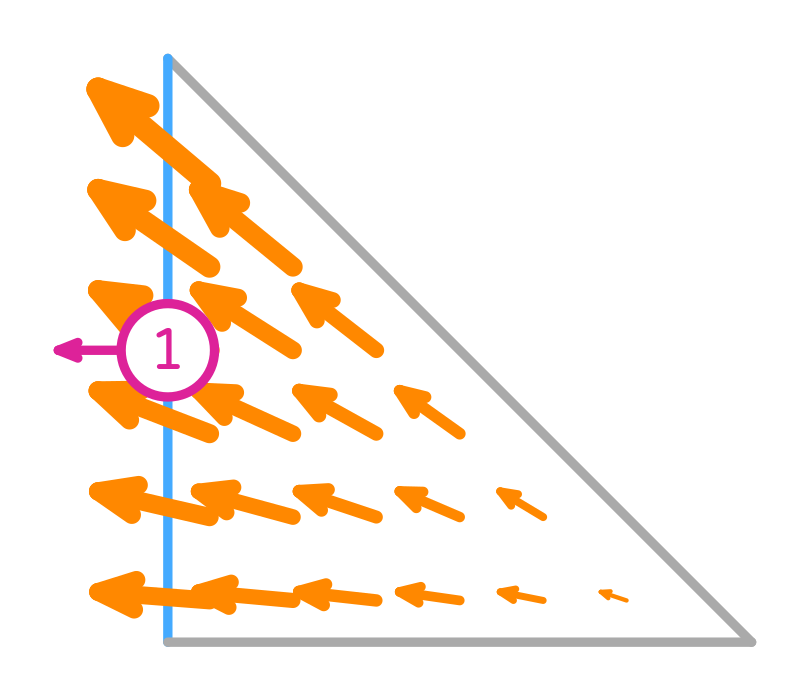
\includegraphics[width=3.3cm]{images/pair_raviart-thomas/element-Raviart-Thomas-variant-equispaced-triangle-1-1-large}
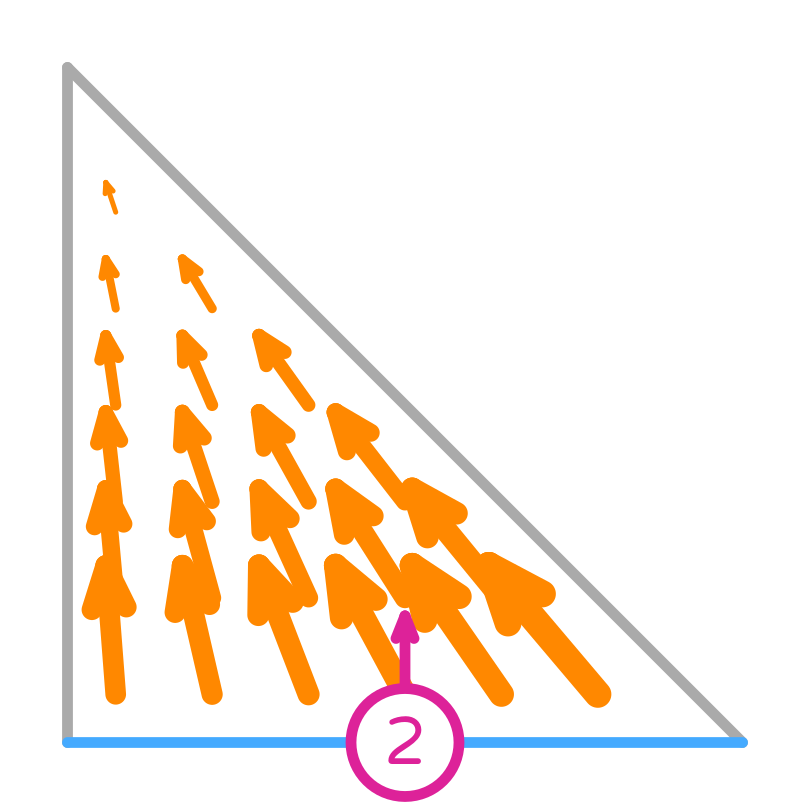
\includegraphics[width=3cm]{images/pair_raviart-thomas/element-Raviart-Thomas-variant-equispaced-triangle-1-2-large}\\
{\captionfont Taken from \url{https://defelement.com/}}
\end{center}

\[
l_0: {\bm v} \rightarrow \int_{e_0} {\bm v} \cdot (1) \hat{n}_0
\]
\[
l_1: {\bm v} \rightarrow \int_{e_1} {\bm v} \cdot (1) \hat{n}_1
\]
\[
l_2: {\bm v} \rightarrow \int_{e_2} {\bm v} \cdot (1) \hat{n}_2
\]
where $e_0$ is the 0th edge and $\hat{n}_0$ is the normal to facet 0,
where $e_1$ is the 1st edge and $\hat{n}_1$ is the normal to facet 1,
where $e_2$ is the 2nd edge and $\hat{n}_2$ is the normal to facet 2.

We have then
\[
{\bm \phi}_0 = \left( \begin{array}{c} -x\\-y  \end{array} \right)
\qquad
{\bm \phi}_1 = \left( \begin{array}{c} x-1\\y  \end{array} \right)
\qquad
{\bm \phi}_2 = \left( \begin{array}{c} -x \\ 1-y  \end{array} \right)
\]
These DOFs are associated with edge 0,1,2 of the reference element.




%-------------------------------------------------------------------------
\noindent
\underline{\bf Degree 1 Raviart–Thomas on a quadrilateral - Lagrange variant}

\begin{center}
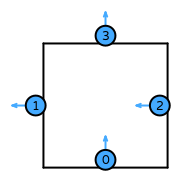
\includegraphics[width=3cm]{images/pair_raviart-thomas/element-NCF-variant-equispaced-quadrilateral-1-dofs}\\
{\captionfont Taken from \url{https://defelement.com/}}
\end{center}

${\cal V}$ is a finite dimensional polynomial space on of dimension $n$ and is spanned by 
\[
\left( \begin{array}{c}1 \\ 0  \end{array} \right),
\left( \begin{array}{c}0 \\ 1  \end{array} \right),
\left( \begin{array}{c}x \\ 0  \end{array} \right),
\left( \begin{array}{c}0 \\ y  \end{array} \right)
\]

Functionals and basis functions:

\begin{center}
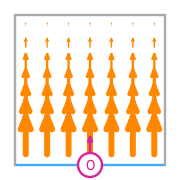
\includegraphics[width=3cm]{images/pair_raviart-thomas/element-NCF-variant-equispaced-quadrilateral-1-0}
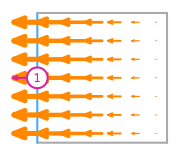
\includegraphics[width=3.5cm]{images/pair_raviart-thomas/element-NCF-variant-equispaced-quadrilateral-1-1}
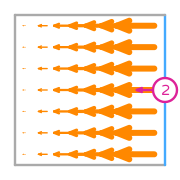
\includegraphics[width=3cm]{images/pair_raviart-thomas/element-NCF-variant-equispaced-quadrilateral-1-2}
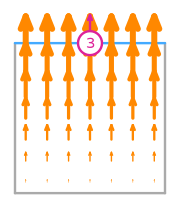
\includegraphics[width=3cm]{images/pair_raviart-thomas/element-NCF-variant-equispaced-quadrilateral-1-3}\\
{\captionfont Taken from \url{https://defelement.com/}}
\end{center}


\[
l_0: {\bm v} \rightarrow \int_{e_0} {\bm v} \cdot (1) \hat{n}_0
\]
\[
l_1: {\bm v} \rightarrow \int_{e_1} {\bm v} \cdot (1) \hat{n}_1
\]
\[
l_2: {\bm v} \rightarrow \int_{e_2} {\bm v} \cdot (1) \hat{n}_2
\]
\[
l_3: {\bm v} \rightarrow \int_{e_3} {\bm v} \cdot (1) \hat{n}_3
\]


where $e_0$ is the 0th edge and $\hat{n}_0$ is the normal to facet 0,
where $e_1$ is the 1st edge and $\hat{n}_1$ is the normal to facet 1,
where $e_2$ is the 2nd edge and $\hat{n}_2$ is the normal to facet 2,
where $e_3$ is the 4th edge and $\hat{n}_3$ is the normal to facet 3.


We have then
\[
{\bm \phi}_0 = \left( \begin{array}{c} 0 \\ 1-y  \end{array} \right)
\qquad
{\bm \phi}_1 = \left( \begin{array}{c} x-1 \\0  \end{array} \right)
\qquad
{\bm \phi}_2 = \left( \begin{array}{c} -x \\ 0  \end{array} \right)
\qquad
{\bm \phi}_2 = \left( \begin{array}{c} 0 \\y  \end{array} \right)
\]
These DOFs are associated with edge 0,1,2 of the reference element.

----------------------------------------

\fullcite{arbf05}


